\newpage

\section{Właściwości}
Siarczek galu występuje w dwóch postaciach:
\begin{itemize}
	\item Siarczek galu(II) - $\mathbf{GaS}$
	\item Siarczek galu(III) - $\mathbf{Ga_{2}S_{3}}$
\end{itemize}

\subsection{Siarczek galu(II)}
$\mathbf{GaS}$ tworzy bezbarwne lub żółte kryształki układu heksagonalnego, grupa przestrzenna
$\mathbf{P\;6_{3}/mmc}$. Kryształ siarczku galu $\mathbf{(GaS)}$ należy do rodziny półprzewodników warstwowych III-VI. Krystalizuje się w sześciokątnej strukturze o parametrach sieci $a = 0,3578$ i $c = 1,547$ nm. Każda warstwa w strukturze krystalicznej składa się z dwóch atomów galu i dwóch atomów siarki ułożonych w stos wzdłuż osi $c$ z powtarzającą się jednostką $\mathbf{S-Ga-Ga-S}$.
\begin{figure}[H]
	\begin{center}
		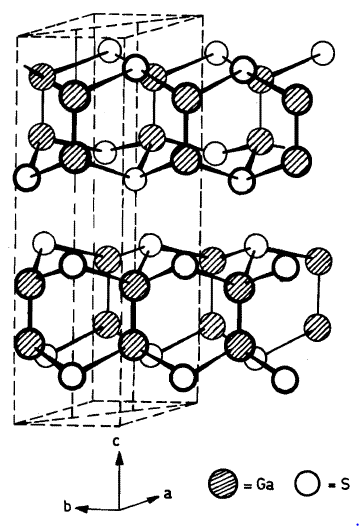
\includegraphics[width=0.5\linewidth]{Wlasciwosci/GaS_Schematic_Structure.png}
		\caption{Schematyczna reprezentacja struktury krystalicznej $\mathbf{GaS}$ [1]}
	\end{center}
\end{figure}
W kryształach $\mathbf{GaS}$ dominują słabe siły van der Waalsa w oddziaływaniach międzywarstwowych. Silne kowalencyjne siły dominują w oddziaływaniach wewnątrzwarstwowych.
$\mathbf{GaS}$ to półprzewodnik szerokopasmowy, który jest obiecującym materiałem. Skośna przerwa energetyczna wynosi $2.5eV$, a prosta wynosi $2.95eV$. Materiał umożliwia
wytwarzanie niebieskich urządzeń emitujących światło [1].

\newpage

\subsection{Siarczek galu(III)}
$\mathbf{Ga_{2}S_{3}}$ jest członkiem III-VI grupy związków chemicznych (III : In Ga VI : S, Se, Te), które mogą posiadać szeroką przerwę energetyczną. 
Nieścisłość pomiędzy atomami III i VI grupy zwykle powoduje, że związek III-VI ma różne stechiometrii, zróżnicowane fazy krystaliczne i różne formy sieci krystalicznej. Jest to półprzewodnik z prostą przerwą energetyczną 2-2.4 eV, i skośną przerwą energetyczną 2.5 - 3.4 eV. Takie rozbieżne wartości wynikają z
niepewności co do jakości kryształu i braku wiedzy struktury Ga2S3.

Struktura krawędzi pasma i pasmo wzbronione są kluczowymi parametrami dla funkcjonalnego półprzewodnika chalkogenkowego
jego zastosowania w optoelektronice, nanoelektronice i urządzeniach fotonicznych.

Materiał $\mathbf{Ga_{2}S_{3}}$ może występować w kilku fazach atomy w których tworzą układy: jednoskośny, heksagonalny, regularny. Może posiadać wadliwą strukturę blendy cynkowej w której $\frac{1}{3}$ miejsc kationowych są puste.
[001-Ga2S3-srep06143]

Faza jednoskośna: a = 1.114, b = 0.641, c = 0.703 nm, $\beta$ = 121.22$^\circ$.[004-Ga2S3-281 - Optik Ga2S3 8]

Znane trzy odmiany $\mathbf{Ga_{2}S_{3}}$:

1) Niskotemperaturowa. Kryształki białego koloru. Układ kubiczny grupa przestrzenna $\mathbf{F\;\overline{4}3m}$.

2) (faza $\beta$) Po podgrzaniu do 550-600$^\circ C$ przekształca się w żółtawą modyfikację, która
tworzy sześciokątną nieuporządkowaną strukturę (typu ZnS(Blenda cynkowa) lub wurcytu). Grupa przestrzenna $P63mc$

3) W temperaturze 600$^\circ C$ tworzą się zasadniczo przezroczyste i jasnożółte kryształki. Jednoskośna struktura. Dla tej struktury około 3.0 eV przerwa energetyczna.

Dla publikacji [001-Ga2S3-srep06143] znaleziono dla fazy jednoskośnej
a = 1.111 b = 0.958 c = 0.640 $\gamma$ = 141$^\circ$ Jednak pozycja znaczących pików na widmie XRD jest taka sama dla każdej fazy
różnica polega jedynie na zmianie względnej intensywności pików dla każdej fazy.
\textbf{Czy z tego wynika że i dla fazy jednoskośnej też są luki?}

Struktura wszystkich faz jest podobna i to jest struktura blendy cynkowej z luką galową na co trzeciej pozycji. Siarka zajmuje
pozycje prawie idealnie sześciokątnego opakowania i różne
uporządkowanie w podsieci kationowej powoduje polimorfizm.	 
[005-Ga2S3-1-s2.0-S0025540816307498-main]

$\mathbf{Ga_{2}S_{3}}$ tworzy jasnożółte kryształki układu jednoskośnego, grupa przestrzenna
$\mathbf{F\;\overline{4}3m}$.
\begin{figure}[H]
	\begin{center}
		\begin{minipage}[h]{0.3\linewidth}
			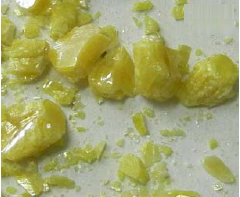
\includegraphics[width=1\linewidth]{Wlasciwosci/Ga2S3_View_Bridgman_Method.png}
		\end{minipage}
		\begin{minipage}[h]{0.3\linewidth}
			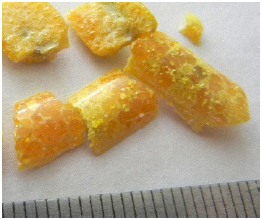
\includegraphics[width=1\linewidth]{Wlasciwosci/Ga2S3_View_Flux_Method.png}
		\end{minipage}
		\caption{Kryształki siarczku galu(III). Po lewej stronie $\mathbf{Ga_{2}S_{3}}$ wytworzony metodą Bridgmana. Po prawej $\mathbf{Ga_{2}S_{3}}$ wytworzony metodą flux-melt.[3]}
	\end{center}
\end{figure}
 Ze względu na budowę warstwową jest rozważany jako perspektywiczny materiał do zastosowań w nanoelektronice i fotonice oraz do generacji sygnałów THz.
 Kryształy $\mathbf{Ga_{2}S_{3}}$ mają również wysoką foto-wrażliwość i silną reakcję luminescencji. 
   Dodatkową jego zaletą jest silna anizotropia optyczna i jest rozważany jako materiał nieliniowy do generacji drugiej harmonicznej (SHG) w zakresie średniej podczerwieni.
\begin{figure}[H]
	\begin{center}
		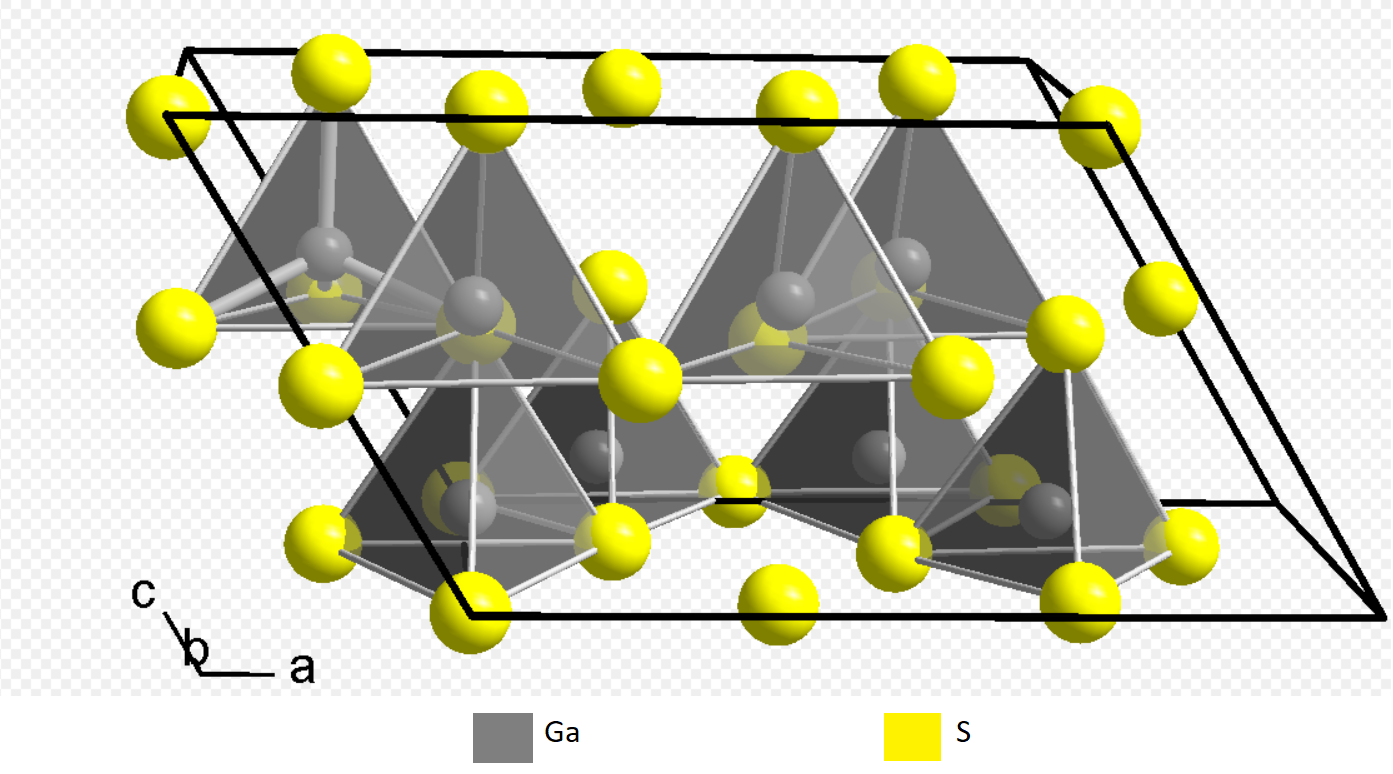
\includegraphics[width=0.6\linewidth]{Wlasciwosci/Ga2S3_Schematic_Structure2.png}
		\caption{Struktura krystaliczna $\mathbf{Ga_{2}S_{3}}$.[2]}
	\end{center}
\end{figure}



